\chapter{Proposta}
\label{chap:proposta}

Neste capítulo, após o embasamento teórico sobre algumas técnicas de modelagem introduzidas no decorrer do Capítulo \ref{cap:fundamentacao-teorica}, o problema será levantado na Seção \ref{sec:problema}. Além disto, na Seção \ref{sec:abordagem}, por meio das ideias apresentadas na Seção \ref{sec:deformacao} e no Capítulo \ref{cap:trabalhos-correlatos}, também será analisada uma abordagem que é pioneira na resolução do problema em questão.

\section{Problema}
\label{sec:problema}

Como ilustrado nas Figuras \ref{fig:domo_castelo}(a) e \ref{fig:domo_castelo}(b), muitas estruturas não retangulares comuns também possuem repetição, neste caso, o arranjo de janelas, blocos e pilares em paredes, torres e domos. Entretanto, uma \textit{shape grammar} baseada em uma caixa padrão não permite a geração de formas nem arranjos arredondados. Apesar de já existirem métodos para modelar ou aproximar formas curvadas ou deformadas, eles ainda apresentam problemas ou falham quando o assunto é a modelagem de formas mais complexas \cite{edelsbrunner2017}. Portanto, se os modelos exigem \textit{designs} curvados, sua criação é trabalhosa, pois as estruturas devem ser aproximadas por geometria plana ou ser colocadas, apropriadamente, com base em objetos pré-modelados \cite{zmugg2014}.

\begin{figure}[h!]
	\centering
	\captionsetup{width=15cm}
	\Caption{\label{fig:domo_castelo} Exemplo arquitetural de um domo e de uma torre de castelo.}	
	\UFCfig{}{
		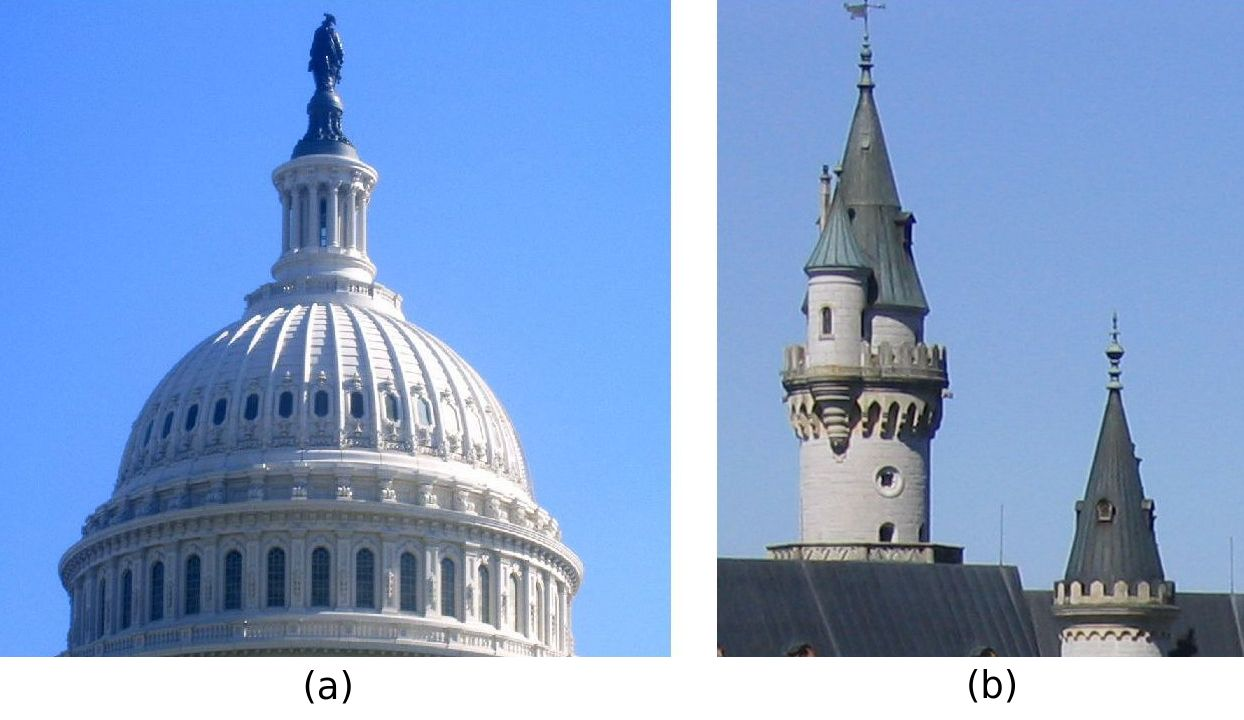
\includegraphics[width=15cm]{figuras/dome_castle.jpg}
	}
	{\Fonte{Adaptado de (a) \citeonline{renee} e (b) \citeonline{susan}}}	
\end{figure}

Conforme mencionado por \citeonline{wonka2018}, uma das limitações de implementação da \gls{SELEX} é justamente a incapacidade de modelar estruturas arredondadas diretamente, trabalhando apenas por meio de sua importação, como complementos, o que impossibilita a modelagem de fachadas curvadas, como a da Figura \ref{fig:selex_limitation}. Assim, na próxima seção, será discutida uma abordagem para resolução deste problema.

\begin{figure}[h!]
	\centering
	\captionsetup{width=15cm}
	\Caption{\label{fig:selex_limitation} Exemplo que está além da capacidade de modelagem da \gls{SELEX}.}	
	\UFCfig{}{
		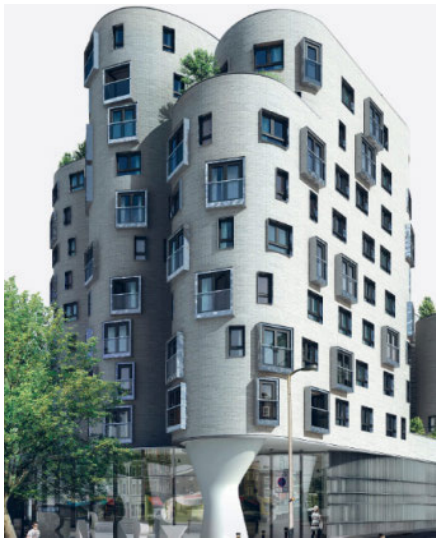
\includegraphics[width=7cm]{figuras/selex_facade_limitation.png}
	}
	{\Fonte{\cite{wonka2018}}}	
\end{figure}

\section{Abordagem}
\label{sec:abordagem}

Nesta seção, será apresentada a ferramenta de modelagem, a descrição do fluxograma de execução, bem como a estrutura do código para geração dos modelos arquiteturais com geometria arredondada, através da \textit{SELEX}, uma linguagem de modelagem contemporânea que introduziu diversas melhorias em relação às suas precursoras.

\subsection{Ferramenta de modelagem}
\label{sec:ferramenta_modelagem}

A implementação da solução a ser apresentada foi realizada no \textit{workspace} de programação do Blender (versão 2.83.8), um \textit{software} de modelagem \textit{open source} mantido pela \citeonline{blender}, utilizando \textit{scripts} escritos em Python, linguagem de programação mantida pela \citeonline{python}.

Os objetos padrões presentes na ferramenta, como plano e cubo, são utilizados para representar, respectivamente, as formas virtuais e de construção, descritas na Seção \ref{sec:selex_definicao_formas}. Cada um destes objetos, por sua vez, possui um conjunto de estruturas de dados que guardam informações sobre a sua representação, tais como quantidade de faces, vértices e arestas, bem como seus identificadores, posições no espaço, dentre outras. Assim, por meio destes atributos, é possível realizar a seleção de determinadas células (faces) ou grupo de células, para que operações de agrupamento, como \texttt{groupRegions}, possam ser aplicadas sobre elas.

O Blender também dispõe de múltiplos artifícios para manipulação de vértices, faces e arestas, em relação a diferentes eixos, conforme mostrado na Figura \ref{fig:blender_coordinates}. Tais recursos são amplamente utilizados em operações como \texttt{addVolume} e \texttt{roundShape}, visando aplicar deformações nos modelos, a fim de gerar arquiteturas arredondadas.

\begin{figure}[h!]
	\centering
	\captionsetup{width=15cm}
	\Caption{\label{fig:blender_coordinates} Representação do sistema de coordenadas do Blender: (a) eixos, (b) vértice, (c) aresta, (d) face.}	
	\UFCfig{}{
		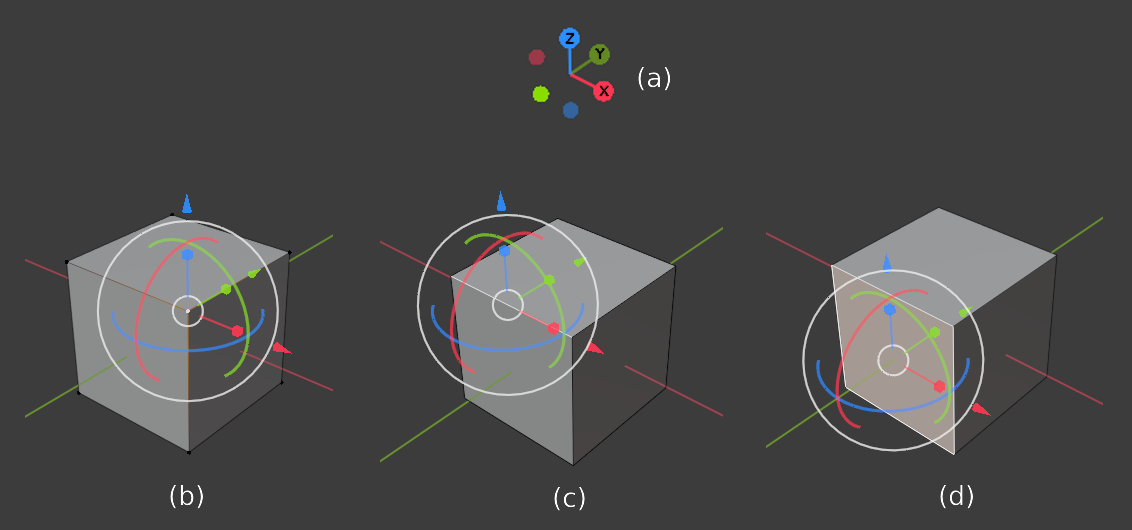
\includegraphics[width=15cm]{figuras/blender_coordinates.png}
	}
	{\Fonte{Próprio autor}}	
\end{figure}

Para fins de depuração, o \textit{software} foi configurado de maneira a prover utilidades extras para desenvolvedores, como a exibição dos índices de faces, arestas e vértices, conforme mostrado na Figura \ref{fig:blender_indices}.

\begin{figure}[h!]
	\centering
	\captionsetup{width=15cm}
	\Caption{\label{fig:blender_indices} Representação dos índices de um objeto: (a) vértices, (b) arestas e (c) faces.}	
	\UFCfig{}{
		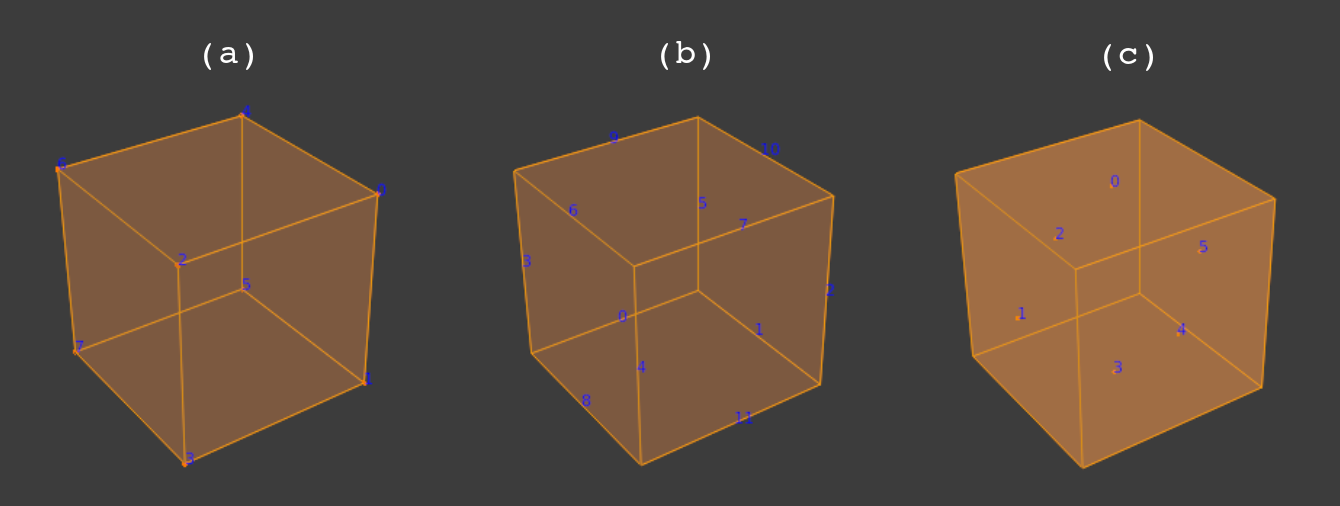
\includegraphics[width=15cm]{figuras/indices_dev.png}
	}
	{\Fonte{Próprio autor}}	
\end{figure}

No processo de geração dos modelos, é utilizada a unidade de medida de comprimento do metro, a qual vem pré-configurada em cada projeto por padrão. Além disto, o panorama adotado para a visualização de cada modelo é mostrado na Figura \ref{fig:axis_values_perspective}, onde (a) representa o lado posterior, (b) representa o lado esquerdo, (c) representa o lado direito, e (d) representa a parte frontal, em relação ao eixos representados em (e).

\begin{figure}[h!]
	\centering
	\captionsetup{width=15cm}
	\Caption{\label{fig:axis_values_perspective} \textit{Wireframe} da representação do lado (a) posterior, (b) esquerdo, (c) direito e (d) frontal, em relação aos (e) eixos cartesianos.}	
	\UFCfig{}{
		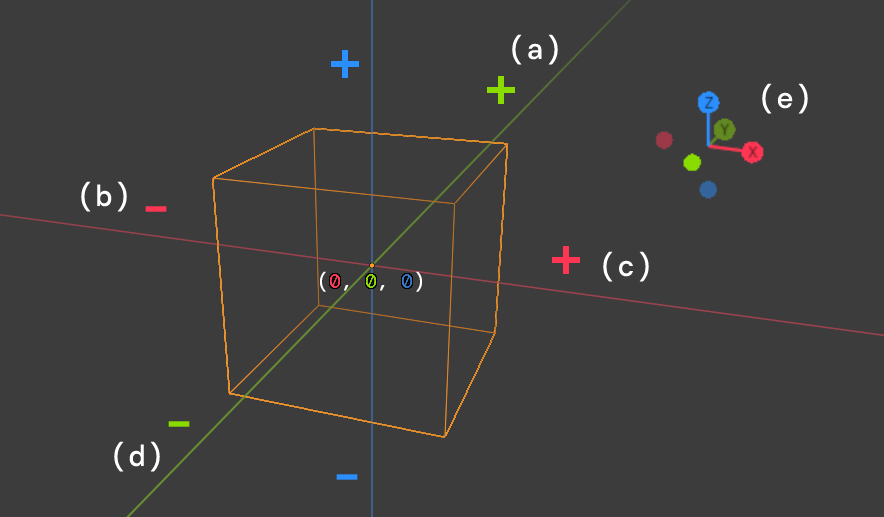
\includegraphics[width=15cm]{figuras/axis_values.png}
	}
	{\Fonte{Próprio autor}}	
\end{figure}

\subsection{Fluxo de modelagem}
\label{sec:fluxo_modelagem}

O fluxograma da Figura \ref{fig:fluxograma}, apresenta um \textit{overview} das etapas que são executadas durante o processo de geração dos modelos, com base no código-fonte disponível no GitHub \footnote{\href{https://github.com/DanielBrito/monografia/tree/main/Codigo-Fonte}{https://github.com/DanielBrito/monografia/tree/main/Codigo-Fonte}}.

\begin{figure}[h!]
	\centering
	\captionsetup{width=15cm}
	\Caption{\label{fig:fluxograma} Fluxograma de execução.}	
	\UFCfig{}{
		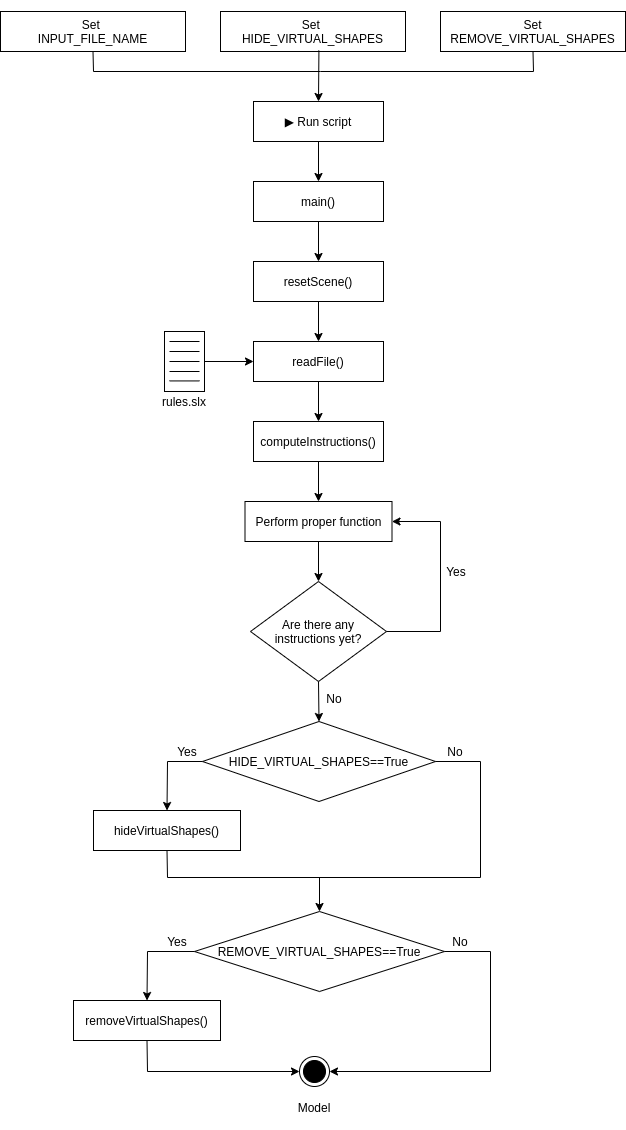
\includegraphics[width=12cm]{figuras/Fluxograma.png}
	}
	{\Fonte{Próprio autor}}	
\end{figure}

Em linhas gerais, inicialmente, deve-se adicionar o arquivo \texttt{main.py} como \textit{script} no \textit{workspace} de programação do Blender. Logo após, deve-se fornecer o nome do arquivo que contém as regras para geração do modelo, podendo ainda serem definidas algumas \textit{flags} para tratamento das formas virtuais ao final do processo, permitindo sua ocultação ou exclusão.

Uma vez que o arquivo com as regras é definido, ao executar o \textit{script}, a função \texttt{main} é acionada, removendo os objetos presentes na cena, e invocando a função de carregamento do arquivo. Durante a leitura das linhas, cada uma das regras é computada e a devida \textit{action} é executada.

Por fim, após a realização de todas as instruções, o modelo final é obtido, podendo ainda ser modificado por meio das ferramentas disponíveis no próprio \textit{software}. Contudo, tais alterações não refletem na árvore de formas, devido ao fato dela ser construída, exclusivamente, através das regras.

Entre as principais operações suportadas pelo presente trabalho estão \texttt{createShape}, \texttt{createGrid}, \texttt{groupRegions}, \texttt{addVolume} e \texttt{roundShape}, as quais serão mais bem detalhadas na próxima seção.

\subsection{Módulos}
\label{sec:modulos}

Nesta seção, além da descrição de alguns detalhes de implementação dos módulos presentes no código-fonte, serão apresentados exemplos básicos do resultado de cada operação de modelagem.

\subsubsection{Imported libraries}
\label{sec:imports}

Informações disponibilizadas pela \citeonline{python} e \citeonline{blender} acerca das bibliotecas utilizadas no presente trabalho:

\begin{itemize}
    \item \textbf{\texttt{bpy}}: Fornece acesso aos dados, classes e funções do Blender, amplamente utilizadas no processo de criação e modificação dos objetos;
    
    \item \textbf{\texttt{math}}: Fornece acesso às funções matemáticas, utilizadas para manipulação de valores numéricos;
    
    \item \textbf{\texttt{os}}: Fornece métodos para utilização de funcionalidades do sistema operacional, como o acesso ao diretório onde se encontra o arquivo com as regras que definem os modelos;
    
    \item \textbf{\texttt{re}}: Fornece operações para correspondência de expressões regulares, utilizadas para extração das informações contidas nas regras, obtidas a partir do arquivo de entrada.
\end{itemize}

\subsubsection{Classes Module}
\label{sec:classes}

Com base no paradigma de Programação Orientada a Objetos, a estrutura é organizada por meio classes, conforme o diagrama da Figura \ref{fig:diagrama_classes}, as quais são utilizadas no gerenciamento da árvore de formas.

\begin{figure}[h!]
	\centering
	\captionsetup{width=15cm}
	\Caption{\label{fig:diagrama_classes} Diagrama de classes referente à estrutura da árvore de formas.}	
	\UFCfig{}{
		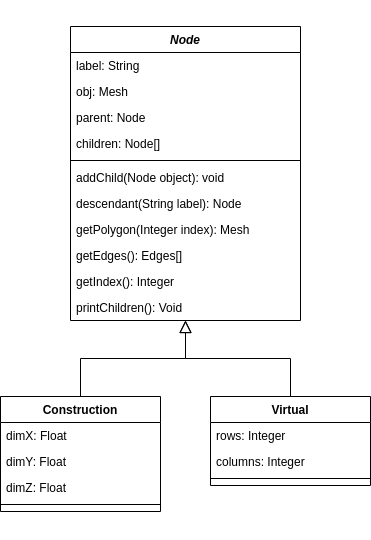
\includegraphics[width=10cm]{figuras/Classes.png}
	}
	{\Fonte{Próprio autor}}	
\end{figure}

Neste caso, \texttt{Node} é a representação genérica de um nó da árvore, já as subclasses \texttt{Construction} e \texttt{Virtual}, são entidades mais específicas, que representam, respectivamente, as formas de construção e as formas virtuais.

\subsubsection{Utility Functions Module}
\label{sec:utilitary_functions}

Definição das principais funções utilitárias que auxiliam no processo de geração dos modelos, por meio da integração com as \textit{actions}:

\begin{itemize}
    \item \textbf{\texttt{create3DMass}}: Invocada durante o processo de execução da \textit{action} \texttt{createShape}, adicionando o modelo de massa padrão, e redimensionando-o de acordo com as configurações definidas nas regras iniciais, por meio dos valores de \texttt{width}, \texttt{depth} e \texttt{height};
    
    \item \textbf{\texttt{vert}} e \textbf{\texttt{face}}: Utilizadas em conjunto durante o processo de execução da \textit{action} \texttt{createGrid}, atuando no posicionamento dos vértices e na criação das faces;
    
    \item \textbf{\texttt{selectNode}}: Invocada para recuperar um nó da árvore de formas, com base nos \textit{labels} presentes nas regras;
    
    \item \textbf{\texttt{placeVirtualShape}}: Trabalha em conjunto com a \textit{action} \texttt{createGrid}, por meio do posicionamento da forma virtual sobre uma determinada face do modelo de massa;
    
    \item \textbf{\texttt{selectToBeVolume}} e \textbf{\texttt{duplicateShape}}: Utilizadas em conjunto para selecionar uma sub-região de uma face do modelo, através de uma forma virtual, a fim de realizar uma extrusão por meio da \textit{action} \texttt{addVolume};
    
    \item \textbf{\texttt{indexRange}}: Utilizada para selecionar um grande intervalo de células, tornando a regra mais sucinta. Conforme especificado na \gls{SELEX}, recebe um índice inicial, um índice final, e retorna como resultado uma lista com os valores no intervalo. Por exemplo, \texttt{indexRange(1,\,5)}, retorna a lista \texttt{[1,2,3,4,5]}.
\end{itemize}

Algumas outras funções também presentes neste módulo são relacionadas ao gerenciamento da cena, como \texttt{resetScene}, que remove os objetos antes da execução das regras; \texttt{hideVirtualShapes}, que oculta as formas virtuais ao final da geração; e \texttt{removeVirtualShapes}, que remove as formas virtuais, com o propósito de gerar um objeto final com menos polígonos, reduzindo o tamanho do arquivo do modelo.

\subsubsection{Actions Module}
\label{sec:actions}

Definição das principais funções que executam as \textit{actions} responsáveis pela geração e manipulação das formas virtuais e de construção, com base nas especificações da \gls{SELEX}. Para exemplificar cada um dos casos, serão utilizadas algumas regras que produzem como resultado final um modelo de massa simples.

Primeiramente, define-se as dimensões do modelo:

\vspace{0.3cm}

\begin{description}
    \item[] \qquad \textit{\#C1: Initial settings}
    \item[] \qquad \textit{label = "building"; width = 9; depth = 11; height = 5;}
\end{description}

\vspace{0.3cm}

Então, por meio da função \texttt{createShape}, que recebe os valores anteriores, o modelo de massa é gerado e a árvore de formas é atualizada, conforme mostrado na Figura \ref{fig:rules_1_c2}.

\vspace{0.3cm}

\begin{description}
    \item[] \qquad \textit{\#C2: Generating mass model}
    \item[] \qquad \textit{\{<> $-$> createShape(label, width, depth, height)\};}
\end{description}

\vspace{0.3cm}

\begin{figure}[h!]
	\centering
	\captionsetup{width=15cm}
	\Caption{\label{fig:rules_1_c2} Modelo de massa inicial.}	
	\UFCfig{}{
		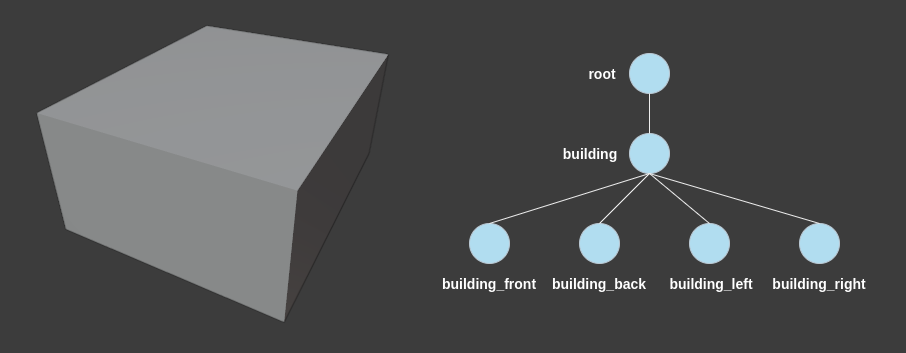
\includegraphics[width=15cm]{figuras/rules_1_c2.png}
	}
	{\Fonte{Próprio autor}}	
\end{figure}

\newpage

A fim de selecionar uma sub-região da parte frontal do modelo, é necessário adicionar uma forma virtual, o que pode ser feito a partir da \textit{action} \texttt{createGrid}, que recebe como parâmetros o \textit{label}, o número de linhas e o número de colunas, produzindo o resultado mostrado na Figura \ref{fig:rules_1_c3}.

\vspace{0.3cm}

\begin{description}
    \item[] \qquad \textit{\#C3: Adding virtual shape}
    \item[] \qquad \textit{\{<descendant()[label=="building"]/[label=="building\_front"]>} \\
    \textit{$-$> createGrid("main\_front\_grid", 3, 7)\};}
\end{description}

\vspace{0.3cm}

\begin{figure}[h!]
	\centering
	\captionsetup{width=15cm}
	\Caption{\label{fig:rules_1_c3} Inclusão de forma virtual.}	
	\UFCfig{}{
		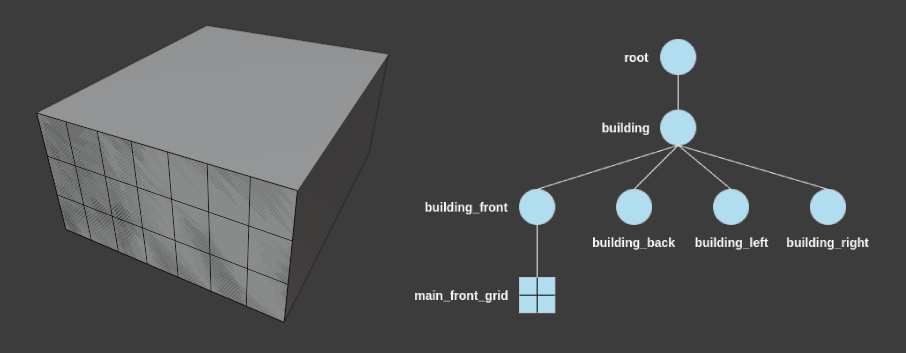
\includegraphics[width=15cm]{figuras/rules_1_c3.png}
	}
	{\Fonte{Próprio autor}}	
\end{figure}

Uma vez que a grade foi criada e devidamente posicionada, torna-se possível selecionar as células desejadas, através dos índices de linha e coluna, com objetivo de realizar operações de agrupamento e extrusão, por meio do \texttt{groupRegions} e da \textit{action} \texttt{addVolume}, respectivamente. Conforme as especificações da \gls{SELEX}, \texttt{addVolume} recebe como parâmetros o \textit{label} do volume a ser produzido, o polígono que sofrerá a transformação, o tamanho da extrusão, e os \textit{labels} das faces laterais do volume gerado. Tal resultado é mostrado na Figura \ref{fig:rules_1_c4}.

\vspace{0.3cm}

\begin{description}
    \item[] \qquad \textit{\#C4: Selecting regions and performing extrusion}
    \item[] \qquad \textit{\{<descendant()[label=="building"]/[label=="building\_front"]} \\
    \textit{[label=="main\_front\_grid"]/[type=="cell"]} \\
    \textit{[rowIdx in (2, 3)] [colIdx in (3, 4, 5)][::groupRegions()]>} \\
    \textit{$-$> addVolume("entrance", "building\_front", 3,} \\
    \textit{["entrance\_front", "entrance\_left", "entrance\_right"])\};}
\end{description}

\vspace{0.3cm}

\begin{figure}[h!]
	\centering
	\captionsetup{width=15cm}
	\Caption{\label{fig:rules_1_c4} Resultado obtido após a operação de extrusão.}	
	\UFCfig{}{
		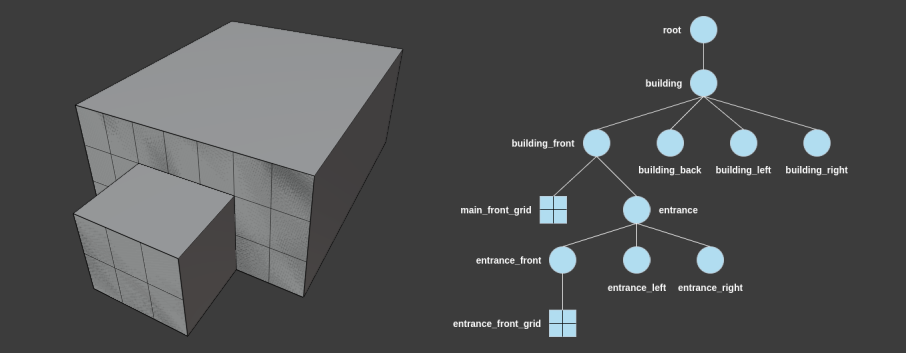
\includegraphics[width=15cm]{figuras/rules_1_c4.png}
	}
	{\Fonte{Próprio autor}}	
\end{figure}

Como proposta, o presente trabalho introduz uma nova \textit{action}, com objetivo de gerar estruturas arredondadas nos modelos. Assim, a operação \texttt{roundShape} pode ser definida da seguinte maneira:

\vspace{0.3cm}

\begin{description}
    \item[] \; \textit{roundShape(type, direction, roundingDegree, segments, sideReference, axis, insideDegree),}
\end{description}

\vspace{0.3cm}

\noindent onde cada um dos parâmetros recebidos desempenha um papel específico:

\vspace{0.3cm}

\begin{enumerate}
    \item \label{itm:type} \textbf{\textit{type}}: Define o tipo de arredondamento, podendo ser classificado como \textit{front}, \textit{left}, \textit{right}, \textit{top} ou \textit{bottom} (Figura \ref{fig:round_type});
    
    \item \label{itm:direction} \textbf{\textit{direction}}: Define a direção do arredondamento, podendo ser classificada como \textit{outside} ou \textit{inside} (Figura \ref{fig:round_direction});
    
    \item \label{itm:roundingDegree} \textbf{\textit{roundingDegree}}: Representa o grau de arredondamento, podendo ser obtido através da divisão do número de colunas selecionadas pela quantidade total de colunas da grade. O mesmo cálculo vale para operações em termos de linhas, visando um arredondamento na horizontal. Por exemplo, na Figura \ref{fig:rules_1_c4}, o modelo possui uma forma virtual com 3 linhas e 7 colunas na região frontal. Portanto, para realizar uma operação de arredondamento vertical na região das colunas 3, 4 e 5, o valor ideal do parâmetro \textit{roundingDegree} é dado por $3/7=0.42$, podendo ainda ser reduzido, a fim de produzir um arredondamento menos acentuado (Figura \ref{fig:round_roundingDegree});
    
    \item \label{itm:segments} \textbf{\textit{segments}}: Representa a quantidade de novos segmentos (faces) a serem criados no processo de deformação da região. Portanto, quanto mais segmentos, maior o grau de realismo. Contudo, também aumenta-se o custo computacional para geração do modelo. É importante ressaltar que deformações do tipo \textit{front} geram o dobro de segmentos, uma vez que atuam nas regiões esquerda e direita, ou inferior e superior, simultaneamente (Figura \ref{fig:round_segments});
    
    \item \label{itm:sideReference} \textbf{\textit{sideReference}}: Referência da direção para qual o vetor normal da região está voltado, podendo assumir valores \textit{main\_front}, \textit{main\_back}, \textit{main\_left} ou \textit{main\_right}, uma vez que a consulta de vértices para operações na região frontal e posterior são efetuadas em relação ao eixo x, mas em operações laterais, utiliza-se como referência o eixo y (Figura \ref{fig:round_sideReference});
    
    \item \label{itm:axis} \textbf{\textit{axis}}: Definido para operações de arredondamento cujo \textit{type} possui valor \textit{front}, podendo ser classificado como \textit{vertical} ou \textit{horizontal} (Figura \ref{fig:round_axis});
    
    \item \label{itm:insideRounding} \textbf{\textit{insideRounding}}: Define o grau de arredondamento interno, sendo $0.05$ por padrão. A diminuição gradativa deste valor, faz a região interna se aproximar cada vez mais de um ângulo reto (Figura \ref{fig:round_insideRounding}).
\end{enumerate}

\vspace{0.3cm}

Então, por meio da introdução deste novo recurso, é possível aplicar uma deformação na sub-região frontal do modelo (Figura \ref{fig:rules_1_c4}), a fim de se obter o resultado da Figura \ref{fig:rules_1_c5}, através da seguinte regra:

\vspace{0.3cm}

\begin{description}
    \item[] \qquad \textit{\#C5: Applying roundShape deformation}
    \item[] \qquad \textit{\{<descendant()[label=="building"]/[label=="building\_front"]/} \\
    \textit{[label=="entrance"]/[label=="entrance\_front"]>} \\
    \textit{$-$> roundShape("front", "outside", 0.42, 30, "main\_front", "vertical")\};}
\end{description}

\vspace{0.3cm}

\begin{figure}[h!]
	\centering
	\captionsetup{width=15cm}
	\Caption{\label{fig:rules_1_c5} Modelo final com estrutura frontal arredondada.}	
	\UFCfig{}{
		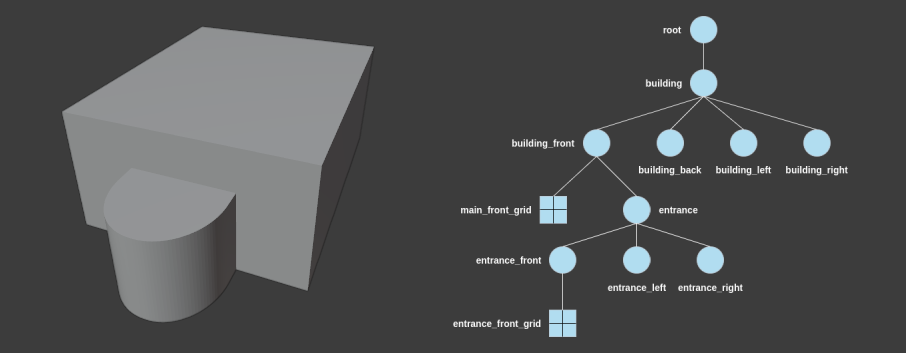
\includegraphics[width=15cm]{figuras/rules_1_c5.png}
	}
	{\Fonte{Próprio autor}}	
\end{figure}

Vale ressaltar que a \textit{action} \texttt{roundShape} atua como uma interface para a operação \texttt{bevel}, um artifício interno do Blender que suaviza bordas e cantos dos objetos.

\newpage

A seguir, serão apresentados outros exemplos ilustrativos com variações de valores para cada um dos parâmetros da \textit{action} \texttt{roundShape}, os quais, em conjunto, são capazes de gerar modelos de massa mais complexos:

\begin{figure}[ht!]
	\centering
	\captionsetup{width=15cm}
	\Caption{\label{fig:round_type} Exemplos de variação do parâmetro (\ref{itm:type}) \textit{type}, com (\ref{itm:direction}) \textit{direction} valorado como \textit{outside}: (a) Forma original, (b) \textit{front}, (c) \textit{left}, (d) \textit{right}, (e) \textit{top}, (f) \textit{bottom}.}	
	\UFCfig{}{
		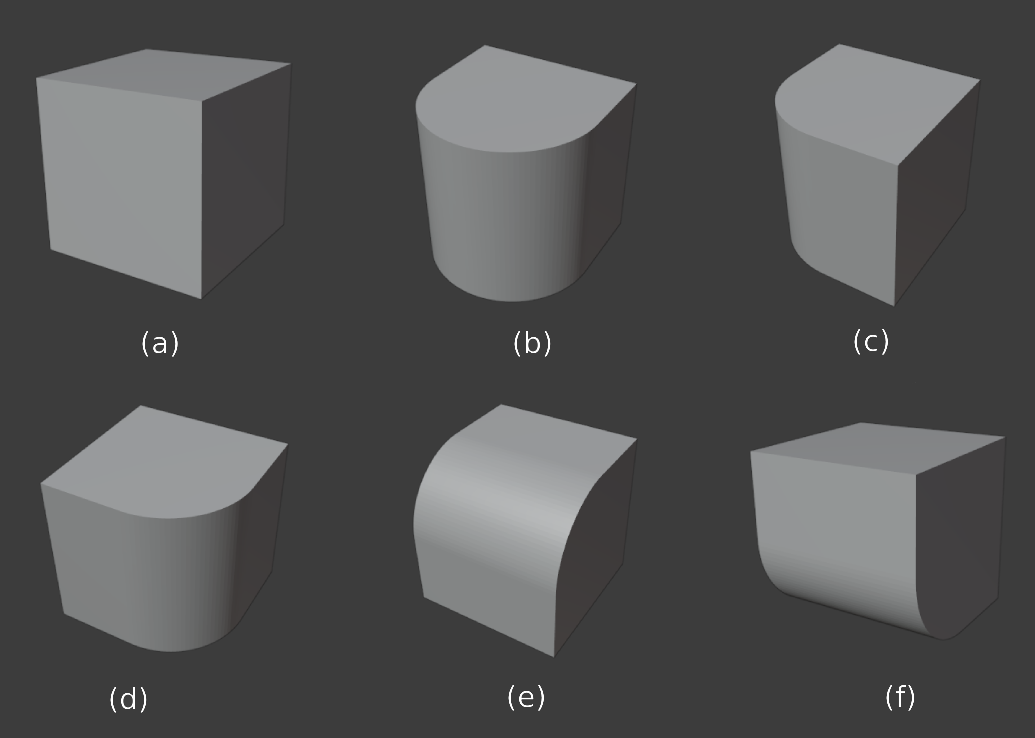
\includegraphics[width=14cm]{figuras/round_type.png}
	}
	{\Fonte{Próprio autor}}	
\end{figure}

\begin{figure}[ht!]
	\centering
	\captionsetup{width=15cm}
	\Caption{\label{fig:round_direction} Exemplos de variação do parâmetro (\ref{itm:type}) \textit{type}, com (\ref{itm:direction}) \textit{direction} valorado como \textit{inside}: (a) Forma original, (b) \textit{front}, (c) \textit{left}, (d) \textit{right}, (e) \textit{top}, (f) \textit{bottom}.}	
	\UFCfig{}{
		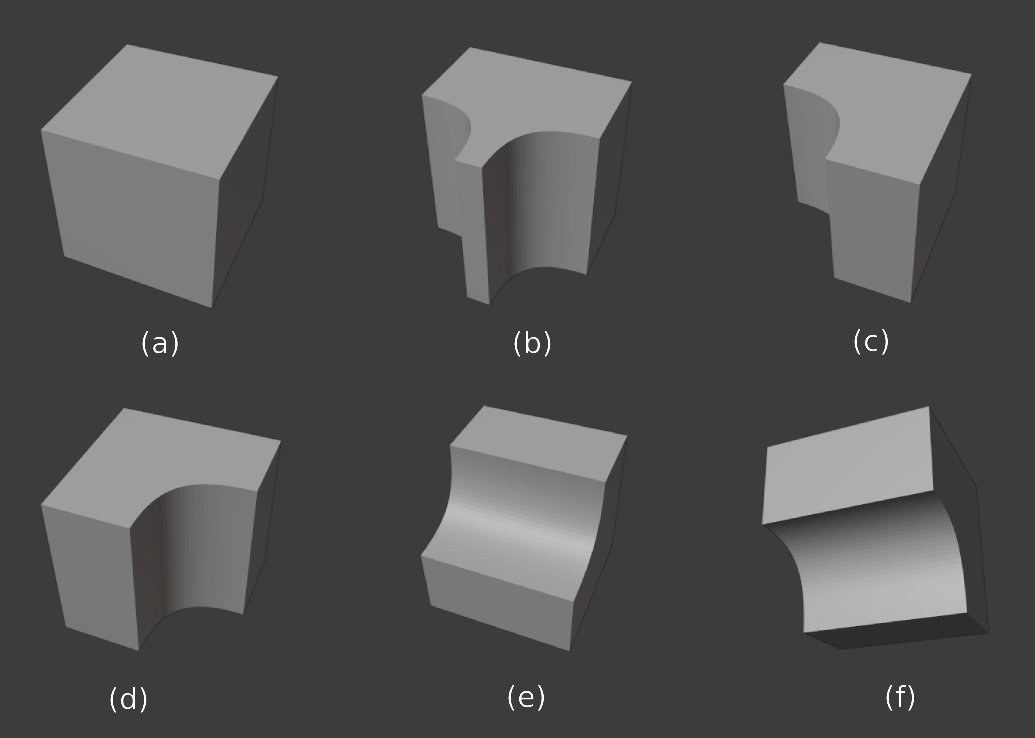
\includegraphics[width=14cm]{figuras/round_direction.png}
	}
	{\Fonte{Próprio autor}}	
\end{figure}

\begin{figure}[ht!]
	\centering
	\captionsetup{width=15cm}
	\Caption{\label{fig:round_roundingDegree} Deformação frontal de um modelo de massa em forma de cubo, possuindo uma grade virtual com apenas uma linha e uma coluna, a partir de diferentes valores de (\ref{itm:roundingDegree}) \textit{roundingDegree}.}
	\UFCfig{}{
		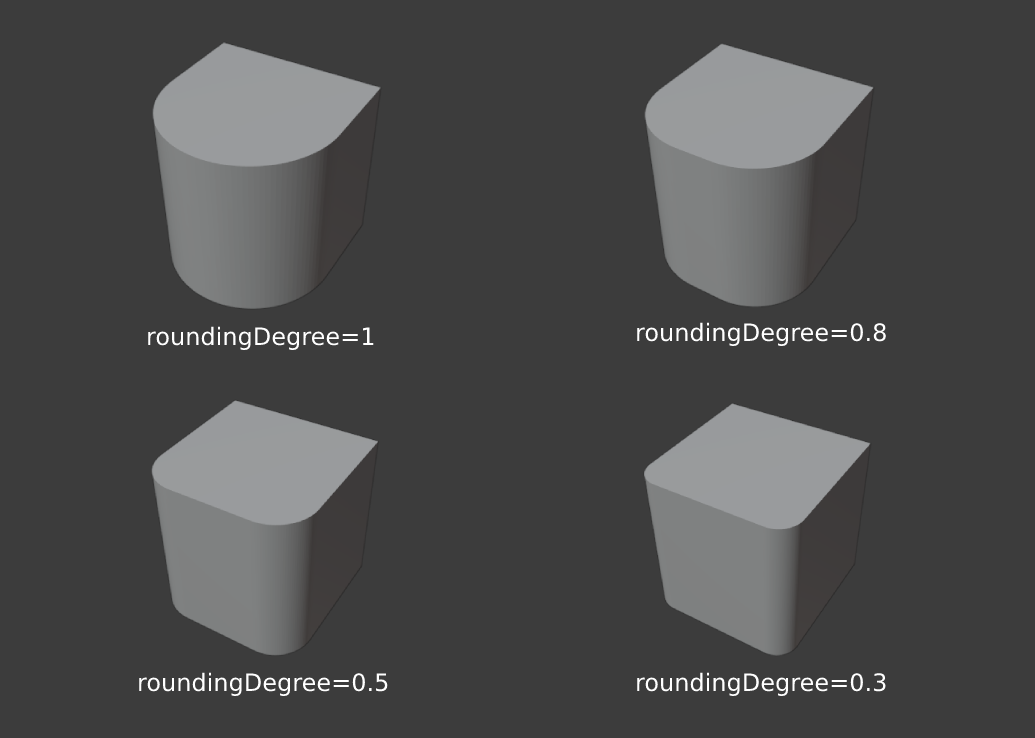
\includegraphics[width=14cm]{figuras/round_roundingDegree.png}
	}
	{\Fonte{Próprio autor}}	
\end{figure}

\begin{figure}[ht!]
	\centering
	\captionsetup{width=15cm}
	\Caption{\label{fig:round_segments} Deformação frontal de um modelo de massa em forma de cubo, a partir de diferentes valores de (\ref{itm:segments}) \textit{segments}.}	
	\UFCfig{}{
		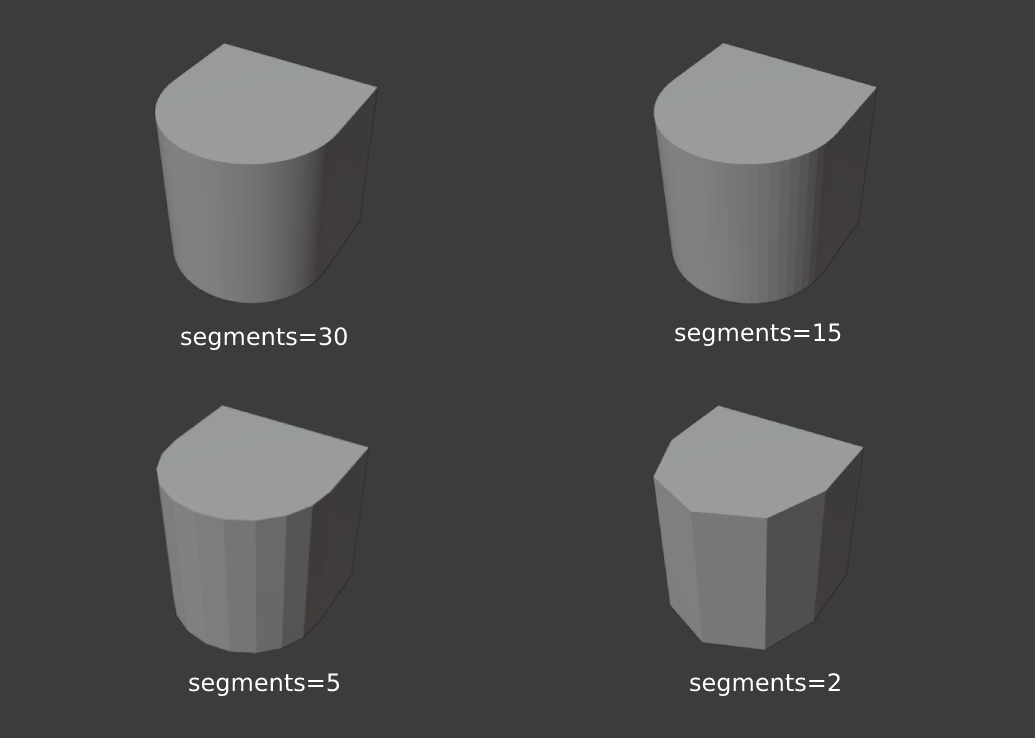
\includegraphics[width=14cm]{figuras/round_segments.png}
	}
	{\Fonte{Próprio autor}}	
\end{figure}

\begin{figure}[ht!]
	\centering
	\captionsetup{width=15cm}
	\Caption{\label{fig:round_sideReference} Representação gráfica dos diferentes valores de (\ref{itm:sideReference}) \textit{sideReference}: \textit{main\_front}, \textit{main\_back}, \textit{main\_left} e \textit{main\_right}.}
	\UFCfig{}{
		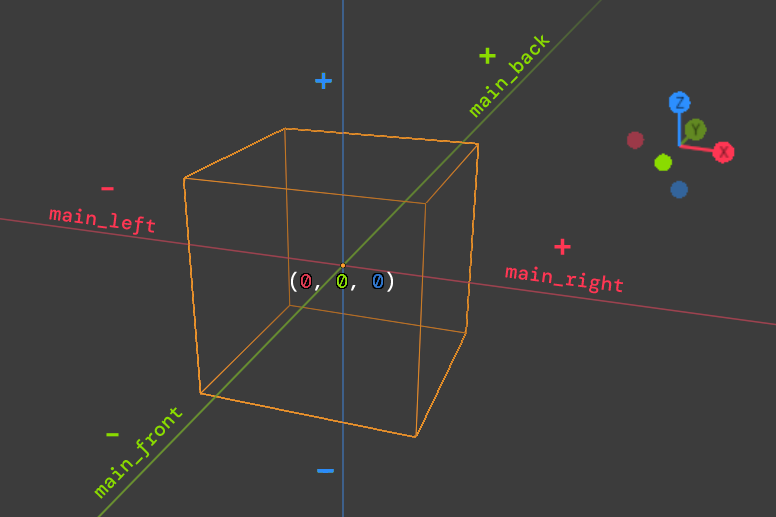
\includegraphics[width=14cm]{figuras/axis_side_ref.png}
	}
	{\Fonte{Próprio autor}}	
\end{figure}

\begin{figure}[ht!]
	\centering
	\captionsetup{width=15cm}
	\Caption{\label{fig:round_axis} Deformação frontal de um modelo de massa em forma de cubo, para diferentes valores de (\ref{itm:axis}) \textit{axis}: (a) \textit{vertical} e (b) \textit{horizontal}.}	
	\UFCfig{}{
		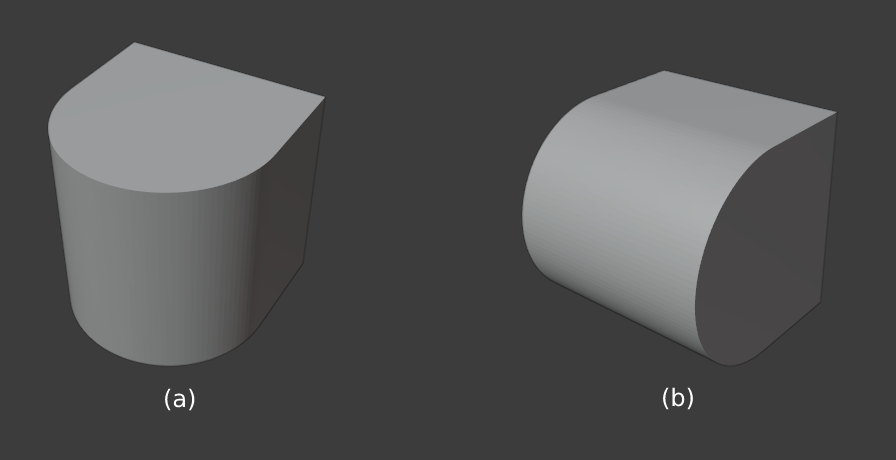
\includegraphics[width=15cm]{figuras/round_axis.png}
	}
	{\Fonte{Próprio autor}}	
\end{figure}

\begin{figure}[ht!]
	\centering
	\captionsetup{width=15cm}
	\Caption{\label{fig:round_insideRounding} Deformação lateral (direita) de um modelo de massa em forma de cubo, possuindo uma grade virtual com apenas uma linha e uma coluna, a partir de diferentes valores de (\ref{itm:insideRounding}) \textit{insideRounding}.}
	\UFCfig{}{
		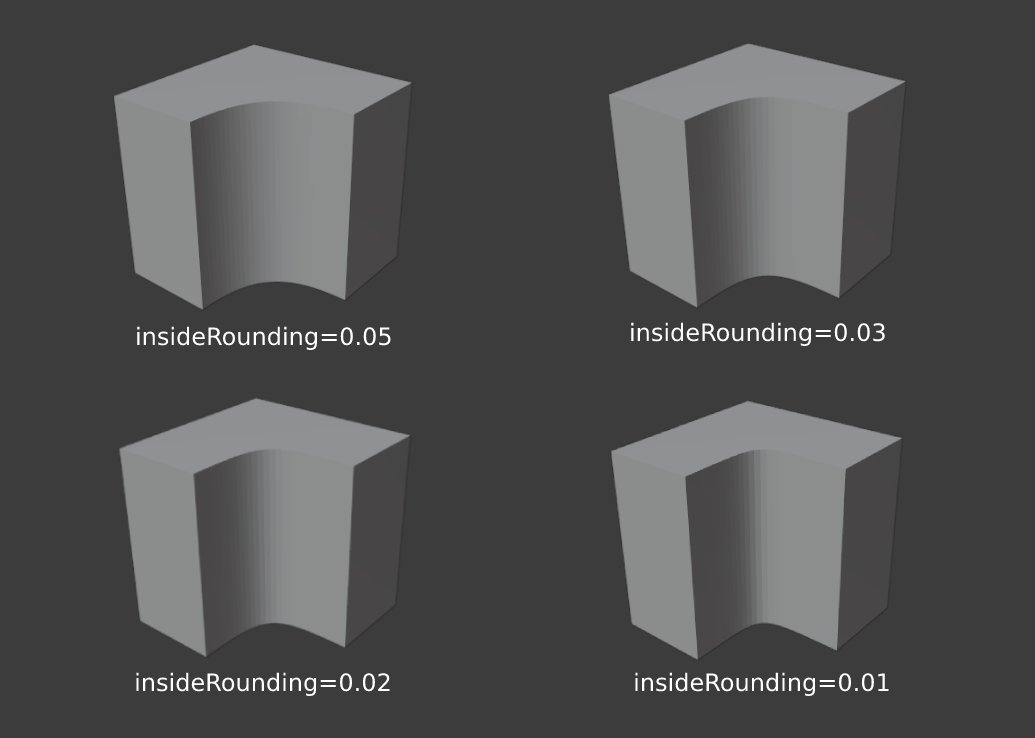
\includegraphics[width=15cm]{figuras/round_insideRounding.png}
	}
	{\Fonte{Próprio autor}}	
\end{figure}

\clearpage

\subsubsection{Outros módulos}
\label{sec:outros_modulos}

No \textit{User Configuration Module}, o usuário informa a \textit{string} referente ao nome do arquivo que contém as regras, sendo atribuída à varivável \texttt{INPUT\_FILE\_NAME}, e também define o estado das \textit{flags} \textit{booleanas} para tratamento das formas virtuais, neste caso, \texttt{HIDE\_VIRTUAL\_SHAPES} e \texttt{REMOVE\_VIRTUAL\_SHAPES}.

No \textit{Input Stream Module}, são definidas as funções responsáveis pela divisão dos \textit{tokens}, com o propósito de extrair os parâmetros a serem passados para as respectivas \textit{actions}:

\vspace{0.3cm}

\begin{itemize}
    \item \textbf{\texttt{loadSettings}}: Utilizada para o carregamento das configurações do modelo de massa, as quais são enviadas para \texttt{createShape};
    
    \item \textbf{\texttt{loadCreateGrid}}: Utilizada para o carregamento das informações referentes às grades virtuais, as quais são enviadas para \texttt{createGrid};
    
    \item \textbf{\texttt{loadAddVolume}}: Utilizada para o carregamento das informações referentes à extrusão de uma determinada região do modelo, as quais são enviadas para \texttt{addVolume};
    
    \item \textbf{\texttt{loadRoundShape}}: Utilizada para o carregamento das informações referentes ao arredondamento de uma determinada região, as quais são enviadas para \texttt{roundShape}.
\end{itemize}

No \textit{File Module}, são especificadas as instruções para leitura do arquivo com base no valor da variável \texttt{INPUT\_FILE\_NAME}. Todas as linhas iniciadas pelo símbolo $\#$ são tratadas como comentários, e o restante são armazenadas em uma lista, a fim de serem enviadas para a função \texttt{computeInstructions}.

No \textit{Execution Module},  é definida a função de inicialização \texttt{main}, utilizada para invocar algumas funções auxiliares, como \texttt{resetScene} e \texttt{readFile}, ou ainda \texttt{hideVirtualShapes} e \texttt{removeVirtualShapes}, se as variáveis \texttt{HIDE\_VIRTUAL\_SHAPES} e \texttt{REMOVE\_VIRTUAL\_SHAPES} possuírem valor \texttt{True}, respectivamente.

\vspace{1cm}

Este capítulo descreveu a problemática e algumas das principais características de implementação do presente trabalho. No próximo capítulo, serão apresentados modelos mais elaborados e uma breve análise estatística da solução proposta.